\begin{section}{Molecular Simulation: History and Importance}

What are the functions of proteins in the body? How can we identify new and better drugs for improved
disease treatment, or optimal materials for designing efficient solar cells?
What are the microscopic mechanisms by which chemicals interact, undergo phase
transitions, or react to form entirely new species? Increasingly, these and other 
essential chemical questions can be addressed with the aid of computer
simulation, 
\cite{VanGunsteren1990,Hospital2015,Chen2015,Karplus2002,Ciccotti2014}
enabling us to, for example, peer into the detailed mechanisms of enzyme catalysis,
\cite{Warshel2003}
watch proteins fold,
\cite{Levitt1975,Lane2013,Piana2014,Perez2016}
virtually screen for novel drug candidates, 
\cite{DeVivo2016}
improve industrial materials,
\cite{Jiang2011,Maurin2016,Bereau2016}
and directly simulate hard-to-understand phase transformations at an atomistic level.
\cite{Kalikmanov2013,Wilding2001}
The question, of course, is: how?


To understand the manner in which computer simulation can be used to obtain obervable experimental properties
of interest,\footnotemark{} we first summarize several fundamental
physical principles
that help define the
fundemand inputs and important techniques required for molecular simulation.
The foundation for molecular simulation comes from the field of
statistical mechanics, where by the mid 19-\super{th} century it was discovered
that experimental observables, which we denote \obs, depend entirely on
a system's temperature, $T$, and the energies available to that system,
%
\begin{align}
\label{eq:intro-boltzmann}
%% \braket{\obs} = \frac{\sum\limits_n \obs_n \exp (-E_n/k_BT)}
%%                     {\sum\limits_n \exp (-E_n/k_BT)}.
\braket{\obs} = 
\frac{\int d\bm p d\bm x \, \obs(\bm p, \bm x) \exp (-H(\bm p, \bm q)/k_BT)}
{\int  d\bm p d\bm x \, \exp (-H(\bm p, \bm x)/k_BT) }
\end{align}
%
Here the angle brackets denote that we're interested in some \emph{average}
value of the observable, $\bm p$ and $\bm x$ denote, respectiely, the momentum
and positions of the particles in the system, 
$H$ defines the classical Hamiltonian describing the potential and kinetic
energy of that system,
and $k_B$ is Boltzmann's constant.\cite{allen1989computer}
Technically,
this expression only holds for classical systems at constant temperature,
however conceptually-similar expressions can be derived outside of these
assumptions. 
%TODO: Cite useful things here
Even though atomic behavior is, in principle, quantum mechanical,
subsequent research over the years have shown that
very satisfactory molecular properties, particularly for heavier atoms at higher
temperatures,
\cite{Karplus2014}
can be obtained by treating molecular systems according to the above classical
description.
As a result of this highly important insight (indeed, Karplus, Levitt, and
Warshel won the Nobel prize in 2013 for these ideas and related
work),\cite{Karplus2014} it becomes possible to use
\cref{eq:intro-boltzmann} to
extract information regarding macroscropic properties of
interest 
given knowledge of the potential and kinetic energies available in a classical
description of the molecular system. 

\footnotetext{
We've been intentionally vague about what these `experimental
properties of interest' might be, as the experimental properties one finds
important vary considerably between applications. 
To offer some concrete examples, drug discovery
studies are often interested in the binding free
energies between proteins and prospective drug
molecules,\cite{DeVivo2016,Bereau2016}
and the optimization of putative solar cell materials often focuses on
open circuit voltages and/or short-circuit currents.\cite{Bereau2016}
}

In practice, most chemical systems contain large numbers of particles, and as the
number of degress of freedom in the system increase, so does the
dimensionality of the integral in \cref{eq:intro-boltzmann}. 
In most practical scenarios, analytical integration is not possible, and for
large systems it is
computationally prohibitive to solve for $\braket{\obs}$ by standard numerical
integration techniques.
\cite{allen1989computer}
In 1953, however a group of
researchers\cite{Metropolis1953} showed how \cref{eq:intro-boltzmann} can be
systematically estimated
$\braket{\obs}$ via appropriate random sampling of the integrand of
\cref{eq:intro-boltzmann} based on a probability distribution $\rho$:
\cite{Harrison2010,allen1989computer}
%
\begin{align}
\label{eq:intro-mc}
\braket{\obs} = \braket{\obs}_{\text{ens}} 
= \lim_{\tau_{\text{obs}} \to \infty} \frac{1}{\tau_{\text{obs}}}
\sum\limits_{\tau = 1}^{\tau_{\text{obs}}}
\obs(\bm{\Gamma}(\tau))
\end{align}
%
In contrast to \cref{eq:intro-boltzmann}, \cref{eq:intro-mc} is the average
over a total number of sampled observations, ${\tau_{\text{obs}}}$, taken of the
system and its properties, 
and $\bm{\Gamma}(\tau)$ denotes the collective positions and
momenta that define the state of the system at each sample point.
The key technique that
defines the resulting \mc algorithm is known as `importance sampling':
provided we cleverly choose our probability distribution, $\rho$, to be
identical to the Boltzmann distribution, $\rho \propto \exp (-H(\bm p, \bm x)/k_BT)$, the
right-hand side of \cref{eq:intro-mc} converges fairly rapidly as a function
of ${\tau_{\text{obs}}}$.  The interested reader is directed to
\citet{allen1989computer} for detailed information on the exact techniques,
algorithms, and practical concerns involved in importance sampling. In
general, however, it is sufficient to know that \mc is one of the main
algorithms used to evaluate average molecular properties,
and that ultimately the \mc technique depends on the accuracy with which we can
evaluate the potential and kinetic energies of a given system.

As an alternative strategy to \mc,
at the turn of the 20\super{th} century
Ludwig Boltzmann proposed his now-famous `ergodic'
hypothesis.\cite{boltzmann1898vorlesungen} This hypothesis states that, over sufficiently
long time periods, the `ensemble average' defined in \cref{eq:intro-boltzmann} becomes
identical to the `time-average' that results from studying the system's
dynamical behavior,
%
\newcommand{\tobs}{\ensuremath{t_{\text{obs}}}\xspace}
\begin{align}
\label{eq:intro-md}
\braket{\obs} = \braket{\obs}_{\text{time}} 
= \braket{\obs(\bm{\Gamma}(t)}_{\text{time}} 
= \lim_{t_{\text{obs}} \to \infty} \frac{1}{t_{\text{obs}}}
\int\limits_0^{t_{\text{obs}}}
\obs(\bm{\Gamma}(t)) dt ,
\end{align}
%
where \tobs indicates the length of time over which we average the system's
properties.\cite{allen1989computer} The
right-hand side of \cref{eq:intro-md} shows that, so long as we know and can
solve for the equations of motion that govern a given system's behavior, we can
simulate the time evolution of that system until the r.h.s. of
\cref{eq:intro-md} converges, thereby obtaining a prediction for
$\braket{\obs}$.
Classical mechanics is
governed simply by Newton's laws of motion,
%
\begin{align}
\label{eq:intro-newton}
- \frac{d E(\bm x)}{d \bm x} \equiv \bm F(\bm x) = m \ddot{\bm x}, 
\end{align}
%
with $m$ a mass, and $\bm F$ the force acting on a
particle. Thus as with \mc, we need only know the potential energy of
the system (and by extension its constituent forces)
in order to solve for the
time-dependent positions, momenta, and (ultimately) properties of a system.
The resulting integration of Newton's equations of motion, a process known
as \md,
has made it possible to study both the kinetic and
thermodynamic properties of a wide range of molecular systems, historically beginning with monatomic
liquids in 1964, and soon leading to the first polymer and protein simulations in 1975 and
1977, respectively.\cite{VanGunsteren1990} Ever since these first studies, and
as a complement to \mc, \md simulation has 
increasingly become a preeminent tool in the investigation and prediction of chemical
phenomena.




%% ========================================================
%% 
%% 
%% 
%% The aim of computer simulations of molecular systems is to compute macroscopic
%% behavior from microscopic interactions.
%% The main contributions a microscopic consideration can offer are (1) the
%% understanding and (2) interpretation of experimental results, (3)
%% semiquantitative estimates of experimental re- sults, and (4) the capability
%% to interpolate or extrapolate experimental data into regions that are only
%% difficultly accessible in the laboratory.
%% \cite{VanGunsteren1990}
%% 
%% The design of materials guided by computation is expected to
%% lead to the discovery of new materials, reduction of materials development
%% time and cost, and the rapid evolution of new materials into products.1
%% \cite{Chen2015}
%% 
%% Simulations can provide the ultimate detail concerning individ- ual particle
%% motions as a function of time. Thus, they can be used to address specific
%% questions about the properties of a model sys- tem, often more easily than
%% experiments on the actual system. For many aspects of biomolecular function,
%% it is these details that are of interest (for example, by what pathways does
%% oxygen enter into and exit from the heme pocket in myoglobin?). Of course,
%% experiments play an essential role in validating the simulation methodology:
%% comparisons of simulation and experimental data serve to test the accuracy of
%% the calculated results and to provide criteria for improving the methodology.
%% This is particularly important because theoretical estimates of systematic
%% errors inherent in simulations have not been possible — that is, the errors
%% introduced by the use of empirical potentials are difficult to quantify
%% ...
%% There are three types of applications of simulation methods in the
%% macromolecular area, as well as in other areas involving mesoscopic systems.
%% The first uses simulation simply as a means of sampling configuration space.
%% This is involved in the utiliza- tion of molecular dynamics, often with
%% simulated annealing pro- tocols, to determine or refine structures with data
%% obtained from
%% experiments, as mentioned above. The second uses simulations to obtain a
%% description of the system at equilibrium, including structural and motional
%% properties (for example, atomic mean- square fluctuation amplitudes) and the
%% values of thermodynamic parameters. For such applications, it is necessary
%% that the simula- tions adequately sample configuration space, as in the first
%% appli- cation, with the additional condition that each point be weighted by
%% the appropriate Boltzmann factor. The third area uses simula- tions to examine
%% the actual dynamics. Here not only is adequate sampling of configuration space
%% with appropriate Boltzmann weighting required, but it must be done so as to
%% correctly repre- sent the development of the system over time. For the first
%% two areas, Monte Carlo simulations can be used, as well as molecular dynamics.
%% By contrast, in the third area where the motions and their development with
%% time are of primary interest, only molec- ular dynamics can provide the
%% necessary information. The three sets of applications make increasing demands
%% on simulation methods as to their required accuracy and precision.
%% \cite{Karplus2002}

\end{section}
\begin{section}{Molecular Simulation: Challenges and Unanswered Questions}

Recent successes in both \mc and \md 
have shown great promise for using molecular simulation in the understanding,
interpretation, and even prediction of experimental
results,\cite{VanGunsteren1990}
making simulation a powerful complement to traditional experimental tools.
\cite{Hospital2015,Karplus2002,Bereau2016,Chen2015,Maurin2016,Jiang2011,Schneider2005,Jorgensen2004}
Nevertheless, accurate and insightful molecular simulation
depends on success in the following three critical aspects of any \md/\mc simulation:
\cite{Lane2013}
%
\begin{enumerate}
\item We must be able to accurately and efficiently quantify the potential
energy, $E_n$, of any state $n$ of the system that might get sampled by the
\md/\mc simulation. 
\cite{Ballone2014,Lopes2015,Saunders2013,DeCarvalho2014}
Henceforth we will collectively refer to these energies, given as a function
of the system state $\bm \Gamma$, as the \pes of a system (Some visual
examples of representative \glspl{pes} are shown in \cref{fig:intro-pes}).
\item We must be able to obtain a representative sample of all states of the system over a sufficiently long timescale
(commensurate with the timescale(s) of the chemical phenomena of interest) so as
to obtain converged property predictions.
\cite{Lei2007,Grossfield2010,Theodorou2010}
This class of problems is often referred to simply as `sampling issues'.
\item Especially when interested in \emph{interpreting} chemical phenomena, we must be
able to analyze the results of a simulation in such a way as to garner
detailed, chemically-intuitive insight into the problem at hand.
\cite{E2010,Pande2010,Rohrdanz2013}
While this task is relatively straightforward for homogeneous liquids and
other `simple' systems,
it can become decidedly
difficult for analyzing complex properties and mechanisms, such as with using
simulation to investigate protein folding mechanisms.
\end{enumerate}
Though our focus in this dissertation will be on the first point (that of
computing potential energies for molecular simulation), all three 
aspects of molecular simulation are challenging in their own right, and form
highly active and important areas of research. 
\cite{Ciccotti2014} 
Moreover, there is significant interplay between these areas in terms of
research development.
As an example, improvements in sampling methods often lead to increased computational
efficiency, thereby enabling use of more accurate (but more costly)
representations of the \pes. Conversely, the next section will discuss how the development of
cost-effective potential energy functions is often necessary for
running simulations over long enough time scales to ensure representative
sampling and robust interpretation of the simulation results. Clearly, insofar
as molecular simulation is concerned, both
accuracy and computational efficiency are of paramount importance. 

%%%%%%%%%%%%%%%%%%%%%%%%%%%%%%%%%%%%%%%%%%%%%%%%%%%%%
\begin{figure}
\centering
    \begin{subfigure}[t]{0.75\textwidth}
        \centering
        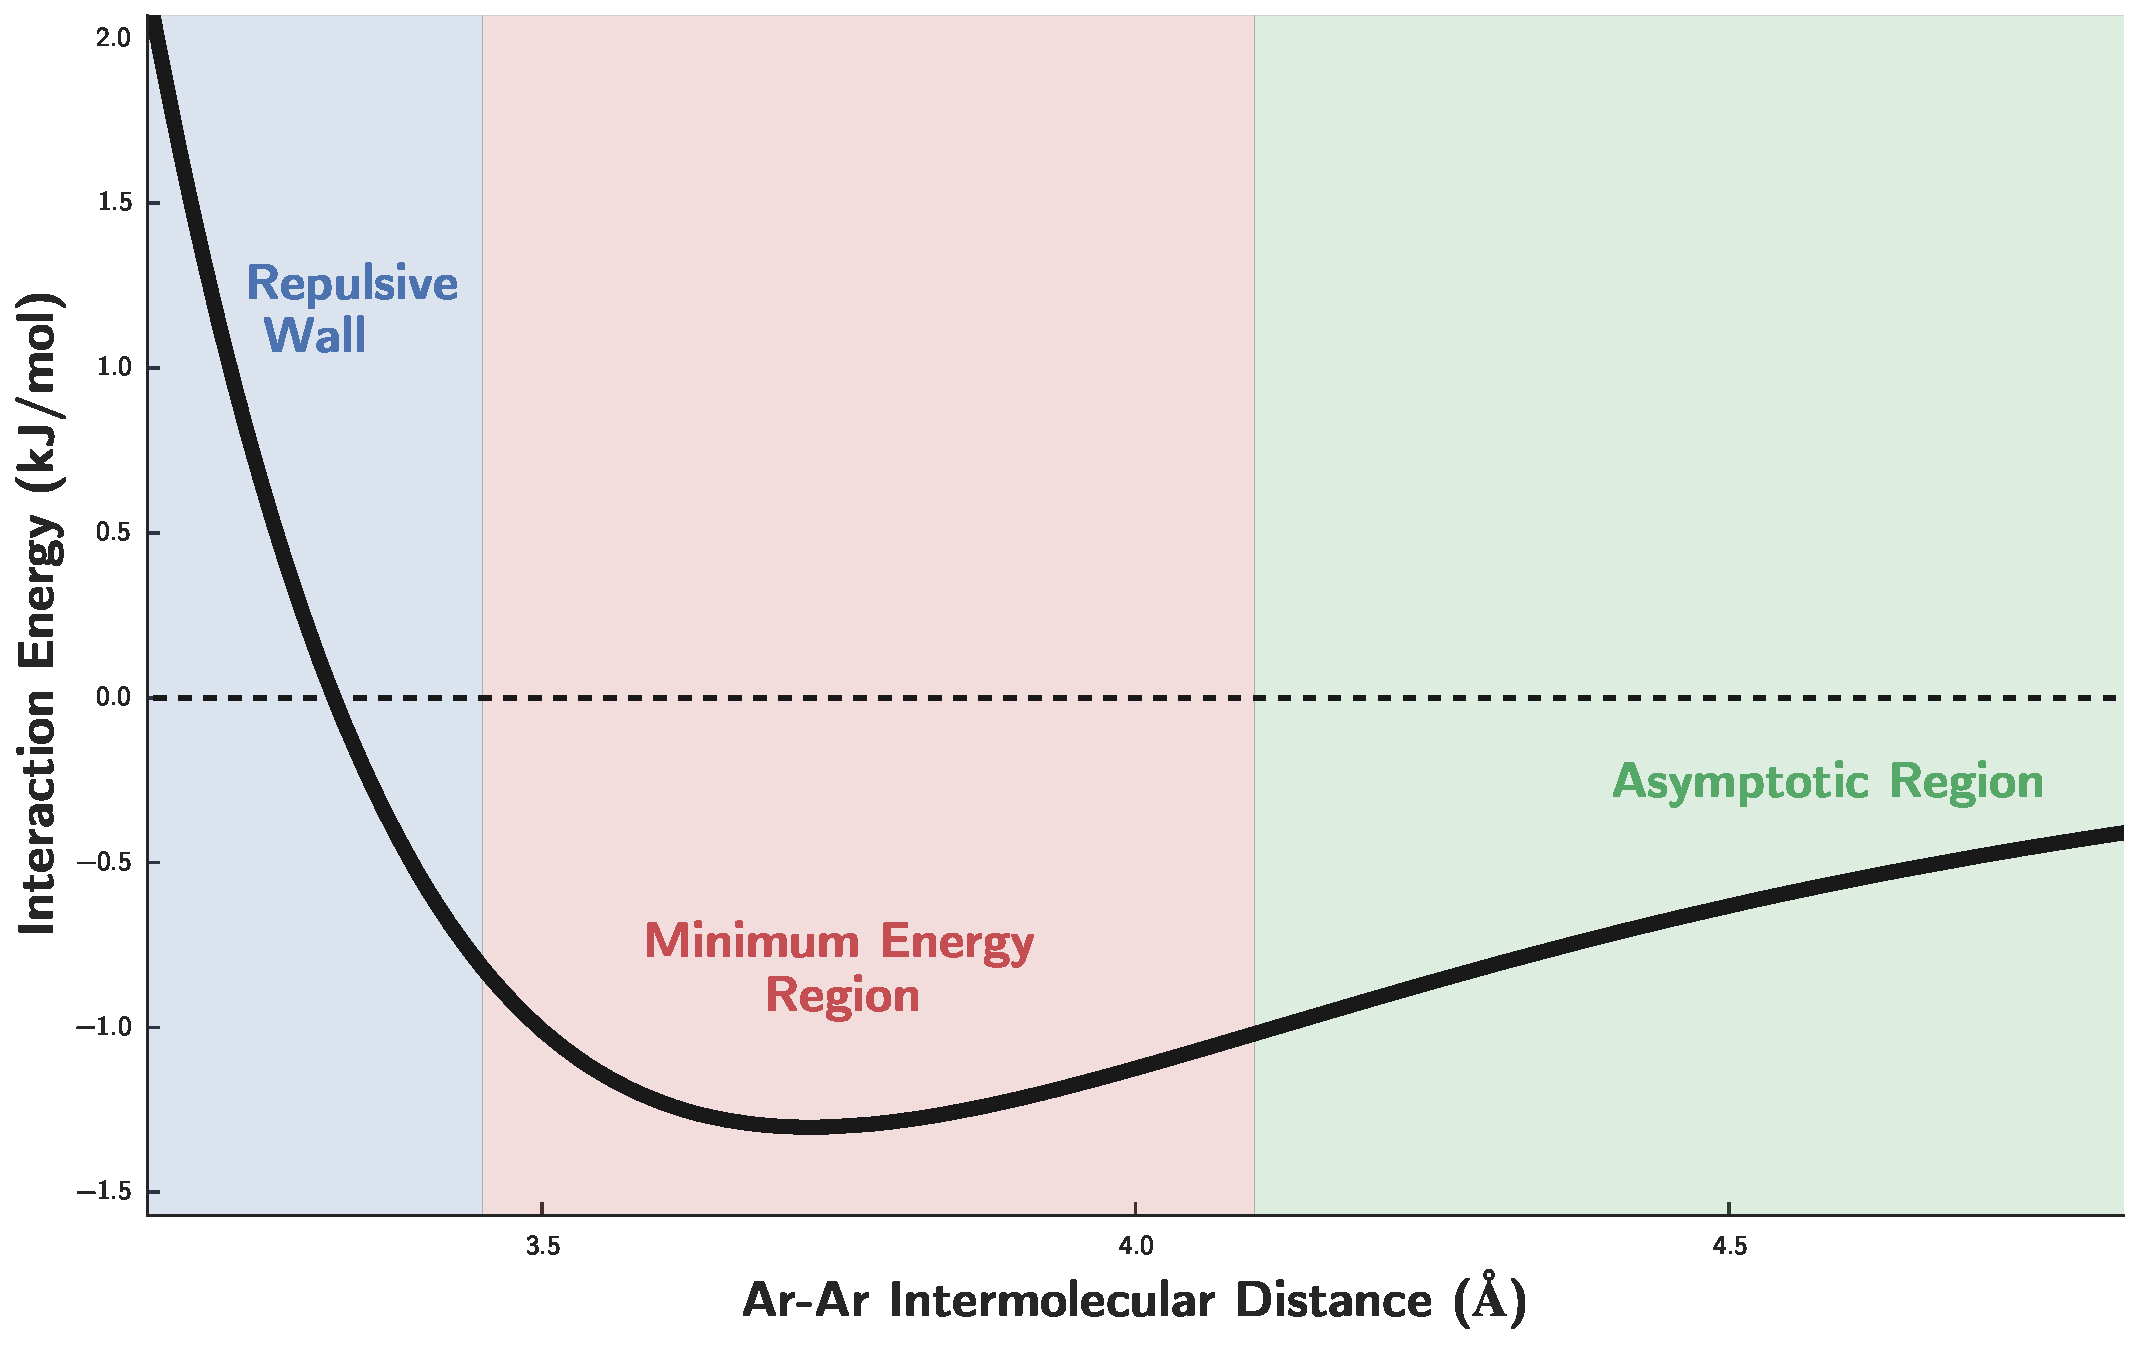
\includegraphics[width=1.0\textwidth]{workflow/generalized_pes.pdf}
        \caption{One-dimensional \pes for the argon dimer.}
    \end{subfigure}
    ~ 
    \begin{subfigure}[t]{0.75\textwidth}
        \centering
        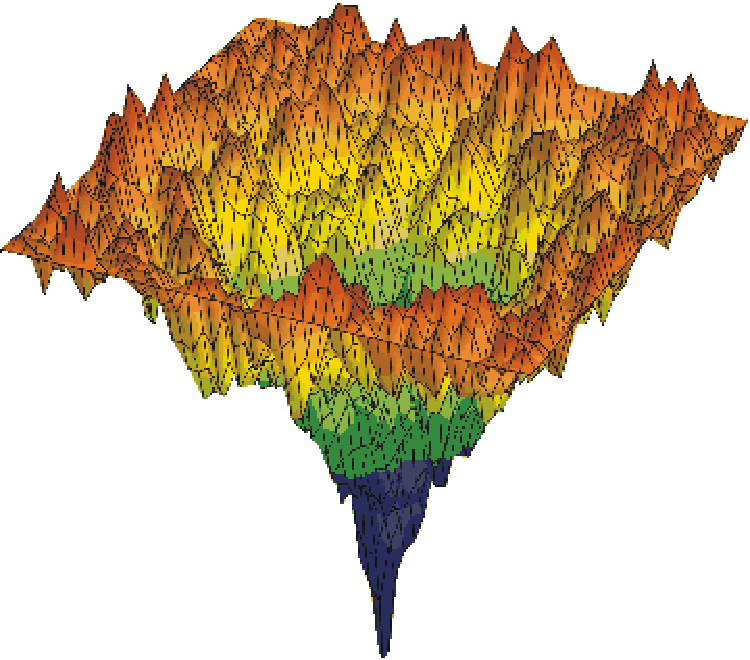
\includegraphics[width=1.0\textwidth]{intro/protein_pes.pdf}
        \caption{Three-dimensional representation of an $N$-dimensional \pes
            for a protein. Copied under a CC license from \citet{Chaplin2017} }
    \end{subfigure}%
\caption{Simple and complex \acrlongpl{pes} for molecular systems.}
\label{fig:intro-pes}
\end{figure}
%%%%%%%%%%%%%%%%%%%%%%%%%%%%%%%%%%%%%%%%%%%%%%%%%%%%%

In the pursuit of increasingly accurate, insightful, and predictive molecular
simulation, it is clear that we must be able to quantitatively represent the
\pes of any molecular system, and, furthermore, that our mathematical
representation of this \pes must be sufficiently accurate and cost-effective so
as to enable simulation that is chemically insightful (given the type of
simulation analysis required for a particular problem or application) and
computationally affordable (in accordance with the length of molecular simulation that will
need to be run in order to appropriately deal with any sampling issues). 
Bearing these stipulations in mind, we can now broadly state the guiding
question for this dissertation: in the pursuit of
accurate and insightful molecular simulation, how can we optimally
obtain a mathematical description of the \pes?

\end{section}
